% !TeX spellcheck = pl_PL
\documentclass[a4paper,twoside]{article}
\usepackage{polski}
\usepackage[utf8]{inputenc}
\usepackage{graphicx}
\usepackage{amsmath}

\usepackage[unicode, bookmarks=true]{hyperref} %do zakładek
\usepackage{tabto} % do tabulacji
\NumTabs{6} % globalne ustawienie wielkosci tabulacji
\usepackage{array}
\usepackage{multirow}
\usepackage{array}
\usepackage{dcolumn}
\usepackage{bigstrut}
\usepackage{color}
\usepackage[usenames,dvipsnames]{xcolor}
\usepackage{svg}
\usepackage{xfrac}
\usepackage{floatrow}

\usepackage{multirow,tabularx}
\newcolumntype{Y}{>{\centering\arraybackslash}X}
\renewcommand{\arraystretch}{2}

% === Reset inkrementacji sekcji przy nowym parcie === %
\usepackage{titlesec}

\makeatletter
\@addtoreset{section}{part}
\makeatother
\titleformat{\part}[display]
{\normalfont\LARGE\bfseries\centering}{}{-60pt}{}

% === Dodanie krpki do sekcji
\titlelabel{\thetitle.\quad}


\setlength{\textheight}{24cm}
\setlength{\textwidth}{15.92cm}
\setlength{\footskip}{10mm}
\setlength{\oddsidemargin}{0mm}
\setlength{\evensidemargin}{0mm}
\setlength{\topmargin}{0mm}
\setlength{\headsep}{5mm}

\setlength{\textfloatsep}{10pt plus 1.0pt minus 2.0pt}


\begin{document}
\bibliographystyle{plain}

% ************************************************************
% --- Strona tytułowa
% ************************************************************
\begin{titlepage}
	\begin{table}[htbp]
		\centering
		\begin{tabular}{|c|c|c|c|c|c|c|}
			\hline
			\multicolumn{7}{|c|}{\textbf{{\LARGE Projekt programistyczny}}} \bigstrut\\[4pt]
			\hline
			Rok akademicki & Termin & Rodzaj studiów & Kierunek & Prowadzący & Grupa & Sekcja \bigstrut\\
			\hline
			\multicolumn{1}{|c|}{\multirow{2}[4]{*}{{\large 2014/2015}}} & \multicolumn{1}{c|}{{\large Wtorek}} & \multicolumn{1}{c|}{\multirow{2}[4]{*}{{\large SSI}}} & \multicolumn{1}{c|}{\multirow{2}[4]{*}{{\large INF}}} & \multicolumn{1}{c|}{\multirow{2}[4]{*}{\begin{tabular}{@{}c@{}}{\large dr inż.} \\[-9pt] {\large Arkadiusz}\\[-9pt] {\large Biernacki}\end{tabular}}} & \multicolumn{1}{c|}{\multirow{2}[4]{*}{{\large GKiO3}}} & \multicolumn{1}{c|}{\multirow{2}[4]{*}{{\large 1}}} \bigstrut\\
			\cline{2-2}    \multicolumn{1}{|c|}{} & \multicolumn{1}{c|}{{\large 12:45 - 15:00}} & \multicolumn{1}{c|}{} & \multicolumn{1}{c|}{} & \multicolumn{1}{c|}{} & \multicolumn{1}{c|}{} & \multicolumn{1}{c|}{} \bigstrut\\
			\hline
		\end{tabular}%
	\end{table}%
	
	\centering
	
\includegraphics[width=0.6\textwidth]{./images/logo.png}
	\\\vspace{10mm}
	\textbf{{\huge Odpowiedzialność klas i interfejsy}}\\\vspace{5mm}
	\textbf{{\Huge Danmaku Shooter}}
	\\
	\vfill
	\begin{flushright}
			{\Large \textbf{Skład sekcji}:}\\
		\begin{tabular}{rr}
			{\Large Buchała} & {\Large Bartłomiej}\\[-3pt]
			{\Large Forczmański} & {\Large Mateusz}\\[-3pt]
			{\Large Motyka} & {\Large Marek}\\[-3pt]
			{\Large Wudecki} & {\Large Wojciech}
		\end{tabular}
	\end{flushright}
	
\end{titlepage}

\part{\huge \textbf{Model interakcji}}

\begin{figure}[h!]
	\hspace{-25mm}
		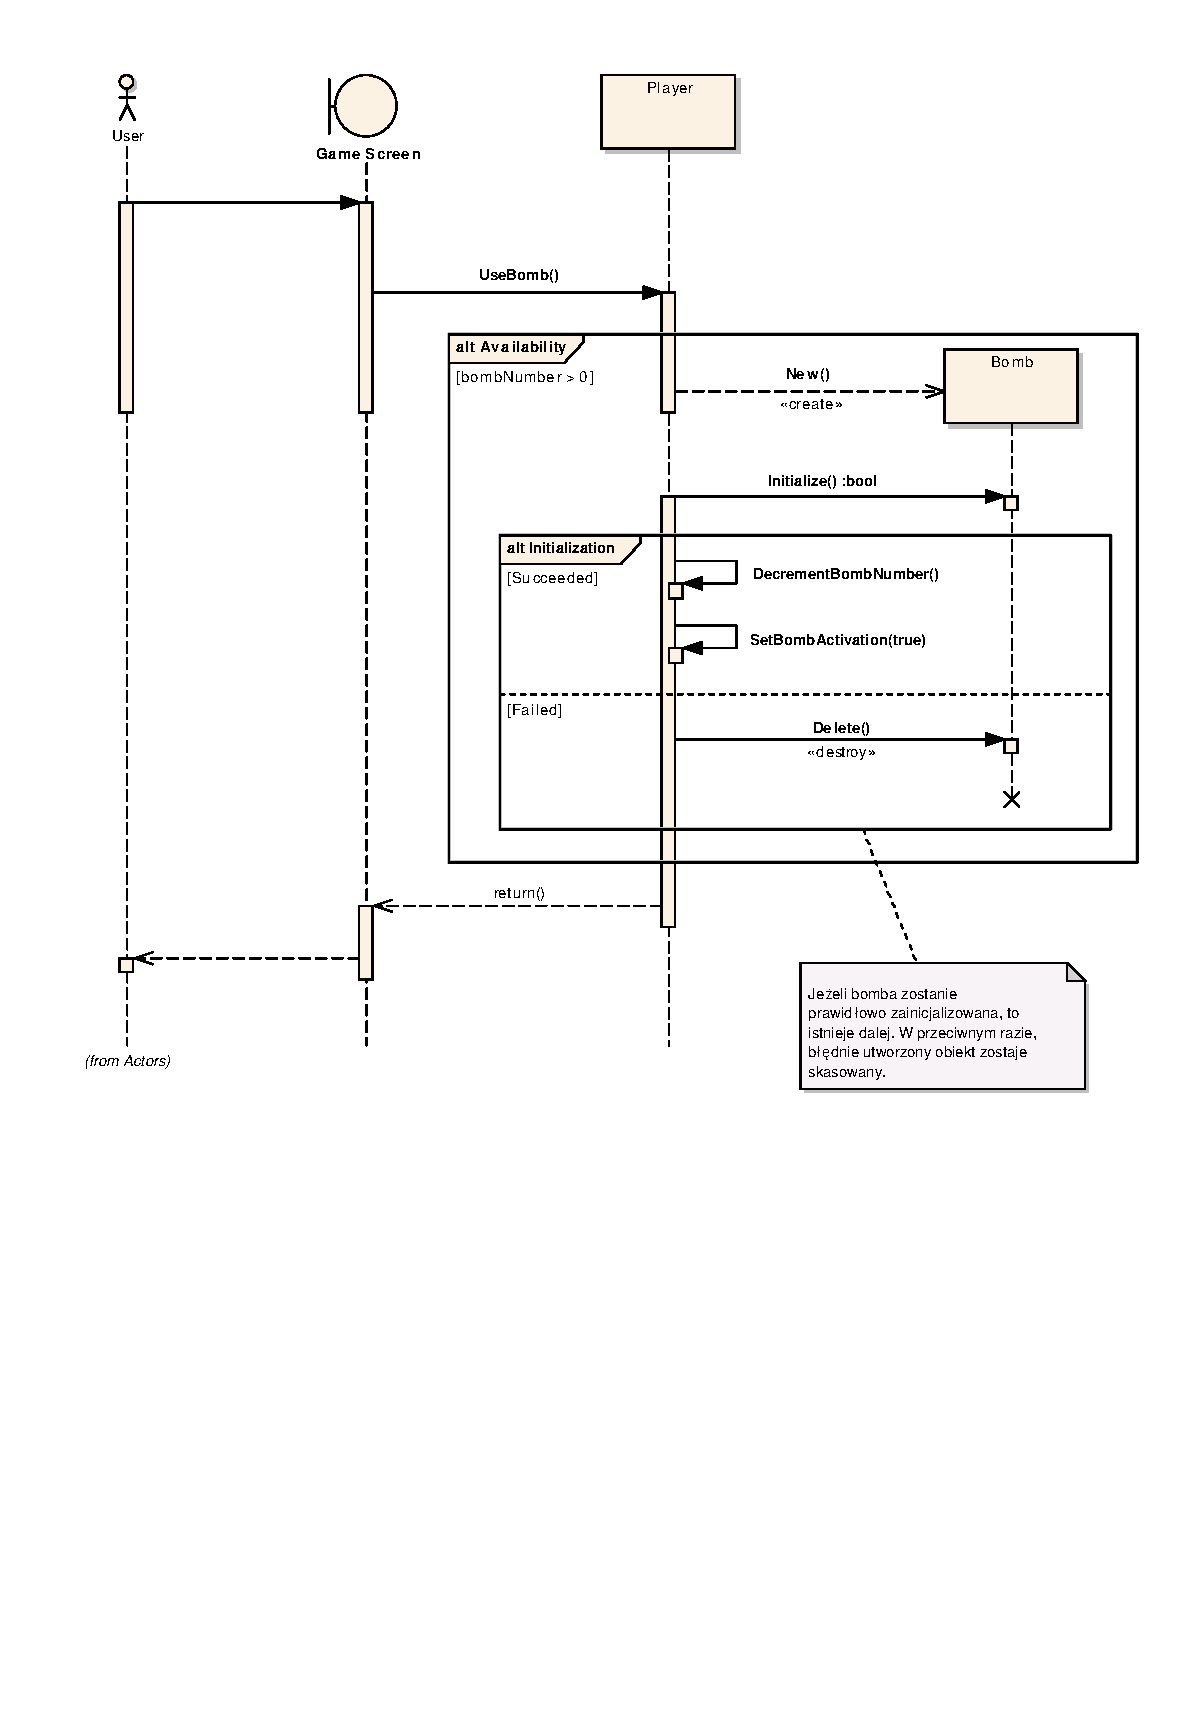
\includegraphics[width=1.15\textwidth, trim={0 10cm 2cm 0}]{./images/Bomba.pdf}
	\caption{{\large Diagram przepływu przypadku użycia bomby}}
\end{figure}

\newpage

\begin{figure}[h!]
	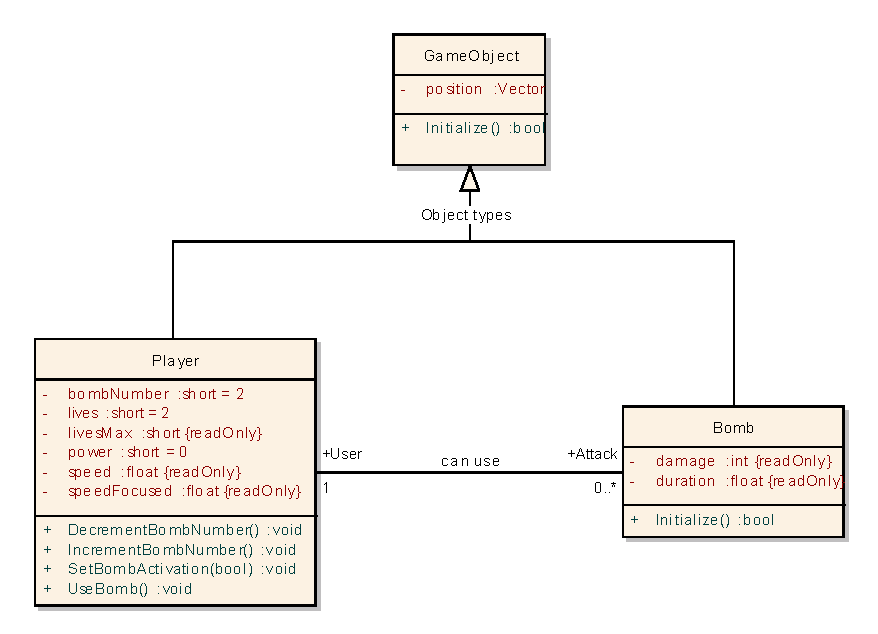
\includegraphics[width=1.1\textwidth]{./images/Fragment.pdf}
	\caption{{\large Fragment diagramu klas}} 
\end{figure}

\vspace*{2\baselineskip}

\part{\huge \textbf{Podmodel klas}}

\section{Klasy użyte w modelu interakcji}

\begin{enumerate}
	
	\item \textbf{Klasa Player}: uniemożliwienie wyjścia graczowi poza planszę, utworzenie trybu \emph{focus}, umożliwienie mu strzelania pociskami i bombami, narysowanie bomby i pocisków, synchronizacja z klasą Input.	
	
	\item \textbf{Klasa Bomb}: implementacja, reakcja na akcję ze strony gracza, narysowanie efektu graficznego, integracja z Timerem (czas trwania bomby, a jej efekt na znajdujące się na mapie pociski/efekt graficzny).
	
\end{enumerate} 

\newpage

\section{Inne klasy}

\begin{enumerate}
	
	\item \textbf{Okno gry}: utworzenie okna w języku WinAPI, inicjalizacja i konfiguracja Direct3D 9, implementacja zegara gry.
	
	\item \textbf{Klasa TitleScreen}: narysowanie ekranu powitalnego, utworzenie menu z wszystkimi możliwościami, utworzenie klasy Menu z szczegółowymi możliwościami zmian, zapisywanie i odczytywanie ustawień z pamięci, utworzenie sprawnego przejścia z ekranu powitalnego do gry i na odwrót.
	
	\item \textbf{Klasa Game}: narysowanie interfejsu gry, wyświetlenie wszystkich danych: liczby żyć i bomb, przechowywanych w klasie Player oraz wyniku i liczby grejzu, przechowywanych w klasie Game, usunięcie pocisków gracza i wrogów z pamięci gdy wyjdą poza planszę, umożliwienie zatrzymania i zakończenia gry, wejścia do menu oraz zapisania wyniku gry do pamięci.		
	
	\item \textbf{Klasa Sprite}: rysowanie sprajtów na ekranie gry, implementacja translacji, skalowania i rotacji, umożliwienie przechowywania i wyboru większej liczby tekstur.
	
	\item \textbf{Klasa Input}: enkapsulacja wszystkich funkcji do obsługi klawiatury, synchronizacja z klasami integralnymi (gra oraz ekran powitalny). Stworzenie uniwersalnych klawiszy – \emph{Shoot}, \emph{Bomb}, \emph{Focus} itp., które będą połączone z odpowiadającymi im wartościami z klasy Input.
	
	\item \textbf{Klasy typu Bullet}: zrealizowanie ruchu pocisków zgodnie ze wskazanymi torami - domyślnie po prostym wektorze, z możliwością zmiany na wskazany tor, umożliwienie przyspieszenia, silna parametryzacja, narysowanie kilku kształtów pocisków w różnych kolorach.

	\item \textbf{Klasy Pattern i Spellcard}: generowanie i układanie wzorów z pocisków, reagowanie na usunięcie pocisków gdy wyjdą poza planszę lub zostaną usunięte przez bombę, realizacja bonusów za pokonanie karty czarów bez straty życia.

	\item \textbf{Klasa Hitbox}: implementacja, narysowanie sprajta hitboxa, zrealizowanie obsługi zdarzeń i styków dwóch hitboxów, wykrywanie \textit{graze} dla hitboxów klas Player i EnemyBullet (poprzez ustawienie pewnej odległości) oraz obsługa utraty życia przy nałożeniu się hitboxów tych klas.
	
	\item \textbf{Klasy typu Bonus}: implementacja, narysowanie sprajtów, synchronizacja z klasami Player (zebranie, zwiększenie powera) oraz Game (zwiększenie wyniku), zwolnienie pamięci po zebraniu przez gracza lub wyleceniu z planszy.

	\item \textbf{Klasa Enemy}: implementacja, umożliwienie strzelania i wykorzystywania patternów, realizacja wrażliwości na pociski gracza, narysowanie sprajtów wrogów.

	\item \textbf{Klasa Stage}: przechowywanie wszystkich obiektów wrogów, decydowanie który jakiego wzoru pocisków używa, silna integracja z timerem – to Stage ma wiedzieć, w której sekundzie pojawiają się wrogowie, kiedy mają strzelić i zejść ze sceny, narysowanie tła.
	
	\item \textbf{Klasa Timer}: implementacja, odliczanie czasu rzeczywistego z określoną częstotliwością, reakcja na zmiany z zewnątrz (przesunięcie okna gry, minimalizajca itp.).
\end{enumerate}

\newpage

\part{\huge \textbf{Specyfikacja interfejsów}}

\section{Drawable}

\begin{itemize}
	\item \textbf{Wykorzystywany w:} Klasie Sprite.
	\item \textbf{Założenie:} Obiekt klasy implementującej ten interfejs może zostać wyświetlany na ekranie 
	\item \textbf{Funkcjonalności:} Metoda Draw() będzie odpowiedzialna za przedstawienie elementu klasy na ekranie. Dodatkowo, implementacja tego interfejsu będzie oznaczała, że klasa będzie powiązana z plikami graficznymi (np. teksturami, modelami 3D).
\end{itemize}

\section{Transformable}

\begin{itemize}
	\item \textbf{Wykorzystywany w:} Klasie Sprite
	\item \textbf{Założenie:} Rozszerzenie klasy Rysowalnej o nowe funkcjonalności.
	\item \textbf{Funkcjonalności:} Klasa używająca interfejsu Transformable będzie mogła dodatkowo wykonać szereg operacji na sprajcie według sposobu zaimplementowanego przez programistę. Rotate() wykona obrót grafiki, Scale() - zmianę rozmiaru, natomiast Translate() przesunie sprajt względem okna aplikacji.
\end{itemize}

\section{IPattern}

\begin{itemize}
\item \textbf{Wykorzystywany w:} wszystkich klasach typu Pattern (Wzorców).
\item \textbf{Założenie:} Zawarcie opisu rozwiązania problemu dla klas typu Pattern.
\item \textbf{Funkcjonalności:} Interfejs służy do automatyzacji procesu tworzenia nowych patternów, narzucajac sposób implementacji, modyfikacji i obsługi kodu źródłowego. Składa się z on 3 metod: inicjalizacji (Initialize()), aktualizacji stanu (Update()) i rysowania(Draw()). Pierwsza z nich określa, ile pocisków zostanie początkowo utworzonych , jakiego typu będą to pociski, ich grafiki itp. Aktualizacja stanu pozwala stwierdzić, jak zmieniają się pociski Patternu w czasie (ruch, obrót, skalowanie). Draw() odpowiada głównie za narysowanie pocisków, pozwalając jednak osobie implementującej na wprowadzenie drobnych zmian.
\end{itemize}

\section{IException}

\begin{itemize}
\item \textbf{Wykorzystywany w:} klasach wyjątków.
\item \textbf{Założenie:} rozszerzenie funkcjonalności wyrzucanych wyjatków.
\item \textbf{Funkcjonalności:} Klasy korzystające z tego interfejsu mają na celu zapobiec jakiemukolwiek błędowi związanemu z obsługą programu, przechwycić go, a następnie poinformować o tym użytkownika i wykonać czynność przewidzianą na wypadek błędu. Implementując ten interfejs, uzyskujemy dodatkowe możliwości podczas wyrzucenia wyjątku przez program: otrzymanie komunikatu i/lub wyświetlenie MessageBoxa. 
\end{itemize}

\newpage

\part{\huge \textbf{Podział zadań}}

\begin{table}[h]
	\begin{tabular}{|l|l|}
		\hline
		\multicolumn{1}{|c|}{\textit{\textbf{Student}}} & \multicolumn{1}{c|}{\textit{\textbf{Klasy do zaprojektowania}}}                                                               \\ \hline
		\textbf{Bartłomiej Buchała}                     & \begin{tabular}[c]{@{}l@{}}a) Klasa Player\\ b) Klasa Game\\ c) Klasy typu Bullet\\ d) Klasa Bomb\end{tabular}                                \\ \hline
		\textbf{Mateusz Forczmański}                    & \begin{tabular}[c]{@{}l@{}}a) Model UML\\ b) Okno Gry\\ c) Klasy Pattern \\ d) Klasa Spellcard\\ e) Klasa Sprite\\ f) Klasa Timer\end{tabular} \\ \hline
		\textbf{Marek Motyka}                           & \begin{tabular}[c]{@{}l@{}}a) Klasa Input\\ b) Klasa Hitbox\\ c) Klasy typu Bonus\end{tabular}                                \\ \hline
		\textbf{Wojciech Wudecki}                       & \begin{tabular}[c]{@{}l@{}}a) Klasa TitleScreen\\ b) Klasa Enemy\\ c) Klasa Stage\end{tabular}                                \\ \hline
	\end{tabular}
\end{table}


\end{document}